\documentclass[12pt,a4paper]{ufpr}
% \usepackage[portuges,brazil]{babel}
% \usepackage[portuguese,brazil]{babel}

%instalar aspell-pt

\usepackage[brazil]{babel}
\usepackage[utf8x]{inputenc}
\usepackage{amssymb,amsmath}
\usepackage{epsfig}
\usepackage{multirow}
\usepackage[table,xcdraw]{xcolor}
\usepackage{lmodern}
\usepackage{textcomp} 
\usepackage[T1]{fontenc}
\usepackage{amssymb}
\usepackage{subfigure}
\usepackage{graphicx}
\usepackage{caption}
\usepackage{setspace}
\usepackage{ps-macros}
\usepackage{comment}
\usepackage{url}
\usepackage{listings}
% \usepackage{psfig}

\newcommand{\specialcell}[2][c]{%
  \begin{tabular}[#1]{@{}c@{}}#2\end{tabular}}

\setcounter{secnumdepth}{3}    % n - numero de niveis de subsubsection numeradas
\setcounter{tocdepth}{3}       % coloca ate o nivel n no sumario

\title{Aplica\c{c}\~oes Escal\'aveis com \textit{MEAN Stack}}
\author{Filipe Leuch Bonfim 000 Michael Liang}
\advisortitle{Orientador} % ou Orientador
\advisorname{Bruno M\"uller Junior.}
\advisorplace{Departamento de Inform\'atica, UFPR}  % departamento, instituicao
\city{Curitiba}
\year{2014}

\banca        % nao insira o nome do orientador, ja eh feito automaticamente
{Prof. ---- }{Departamento de Inform\'tica, UFPR}
{Prof. ---- }{Departamento de Inform\'tica, UFPR}
{}{} % se nao houver deixe em branco {}{}
{}{}    % se houver um quarto membro na banca, inserir nome e instituicao

\defesa{22 de dezembro de 2014} % dia em que foi realizada a defesa da dissertacao

\begin{document}

%\makecapaproposta              % cria capa para proposta%
\makecapadissertacao            % cria capa para dissertacao de mestrado %
%\makerosto                     % cria folha de rosto para versão final da UFPR %
%\maketermo                     % cria folha com o termo de aprovação da dissertação%

%\singlespacing           % espacamento 1 - capa UFPR%
%\onehalfspacing          % espacamento 1/2 %
\doublespacing            % espacamento 2 - UFPR %

\pagestyle{headings}
\pagenumbering{roman}

%\chapter*{Agradecimentos}
%\input{agradecimentos.tex}          % possiu somente o texto

\tableofcontents

\listoffigures         % se houver mais do que 3 figuras
\addcontentsline{toc}{chapter}{\MakeUppercase{Lista de Figuras}}
\newpage

%\listoftables        % se houver mais do que 3 tabelas
%\addcontentsline{toc}{chapter}{\MakeUppercase{Lista de Tabelas}}
%\newpage

\chapter*{Resumo}
\addcontentsline{toc}{chapter}{\MakeUppercase{Resumo}}
%Texto do resumo....
	Nos últimos anos, tem-se observado um grande crescimento na utilização de sistemas robóticos no dia a dia.
	Cada vez mais pesquisadores em robótica têm se concentrado no desenvolvimento de robôs móveis, fazendo com que os
	 robôs possam se mover e interagir com o ambiente de forma autônoma, 
	o que abre um vasto campo de novas aplicações e, consequentemente, muitos desafios, como:  localização, construção de mapas e o problema
	de auto localização e construção 
  de mapas de ambiente simultâneos(\textit{Simultaneous Localization and Map Building - SLAM}). 
		
    Este trabalho propõe um sistema de localização para robôs móveis, 
    baseado no método empírico sugerido no artigo \cite{wifiRadar},
    que provê a localização de um terminal móvel em um ambiente \textit{indoor}. 
    O método é baseado na força do 
    sinal recebido(\textit{Received Signal Strength} - RSS), que é muito explorada em
    em técnicas de localização em uma rede de sensores sem fio pela fácil aplicabilidade. Serão apresentadas também, outras 
    técnicas utilizadas na localização em uma rede de sensores sem fio.
  
	Todo o sistema foi desenvolvido na plataforma Android, pela sua fácil incorporação à robótica devido ao 
	grande quantidade de sensores suportados. Serão brevemente comentadas
	algumas características deste sistema operacional e de uma aplicação Android.
   
   Os resultados obtidos pelo sistema proposto mostram que:
      \begin{itemize}
      \item 22,8\% das estimativas possuem precisão de 1 metro ou menos.
      \item 77,1\% das estimativas possuem precisão de 3 metros ou menos.
      \item 91,4 \% das estimativas possuem precisão de 5 metros ou menos.
     \end{itemize}
	
\textbf{Palavras-chave:} RSS, Localização, RSS fingerprint, Robós Móveis, Android, WSNs.           % somente o texto
\newpage

\chapter*{Abstract}
\addcontentsline{toc}{chapter}{\MakeUppercase{Abstract}}
  
  \textbf{Keywords:} MEAN, Javascript, Node.js, Angular.js, MongoDB, Express.js, Scalability.        % somente o texto
\newpage


\pagenumbering{arabic}

\chapter{Introdu\c{c}\~ao}
\label{Introducao}

% Atualmente a sociedade possui uma ligação muito forte com a internet. A cada segundo muitas pessoas acessam a rede mundial de computadores, e com essa quantidade grande de acessos as plataformas webs necessitam suportar esses acessos simultâneos sem ter problemas, pois qualquer entropia\footnote{Segundo a teoria geral dos sistemas, entropia é consequência da falta de relacionamento entre as partes de um sistema, o que provoca perdas e desperdícios} pode ser considerado um prejuízo para quem depende desta tecnologia. Por isso quando alguém necessitar criar uma aplicação web para suportar múltiplos acessos simultâneos, esta pessoa decidirá pela melhor aplicação escalar para seu problema, uma solução possível é através de um conjunto de ferramentas conhecidas como MEAN que serão abordadas nesta monografia.
Uma aplicação web pode ser resumida em requisições de um cliente ao servidor. Após o servidor ter recebido a requisição, ele envia uma resposta ao cliente. Esta resposta pode ser desde uma página HTML até uma página de erro.

Considere a seguinte situação, muitos clientes requisitando uma página HTML ao mesmo tempo e o servidor tendo que responder a todos eles. Se o servidor tratar esses pedidos como uma fila e somente responder a próxima requisição quando a anterior estiver terminada, os clientes que tiveram suas requisições no fim desta fila, terão maior tempo de resposta implicando em demora para carregar a página do lado do cliente.

Para diminuir o tempo de duração de múltiplas requisições de clientes ao servidor, existem diversas soluções que utilizam técnicas de escalabilidade, alguns exemplos são melhorar o hardware do servidor, com a substituição do hardware antigo por um mais moderno com um poder de processamento maior, e no caso do software, é checar se as ferramentas que estão sendo utilizadas possuem sinergia e foram desenvolvidas para serem escaláveis.

A proposta deste texto é apresentar uma solução via software que visa ajudar a resolver o problema de escalabilidade. O MEAN \textit{Stack}. O MEAN é um acrônimo das quatro tecnologias que são o banco de dados MongoDB, o Node.js e o Express.js na parte do servidor e por último o AngularJS no lado do cliente.

\section{Objetivo}

Nesta monografia serão apresentados conceitos e funcionalidades de um conjunto de tecnologias com o foco em resolver os problemas de aplicações web altamente escaláveis. Esse conjunto é conhecido como MEAN \textit{Stack}\footnote{\textit{Stack} no sentido de pilha, no caso uma pilha de aplicações.}, que é basicamente a utilização de quatro tecnologias baseadas em Javascript: \textbf{M}ongoDB, \textbf{E}xpress.js, \textbf{A}ngularJS e \textbf{N}ode.js. Será apresentado como o MEAN \textit{Stack} lida com a escalabilidade e como é o desempenho de alguns de seus componentes, através da análise de testes de desempenho.

Para demonstrar como uma aplicação MEAN é implementada e como seus componentes interagem entre si foi desenvolvida uma aplicação usando MEAN \textit{Stack} e o Socket.io  baseada na aplicação \textit{Math Race}. A idéia do \textit{Math Race} é realizar uma competição em tempo real para ver qual jogador acerta mais contas de matemáticas em determinado tempo. A partir desta implementação, testes de escalabilidade foram feitos para análise dos resultados.

\section{Organização do trabalho}

Este trabalho está dividido em quatro partes. A primeira parte trata os conceitos que foram utilizados para o desenvolvimento do tema, como aplicações web escaláveis, programação orientada a eventos, Javascript e NoSQL. 

Na segunda parte explicamos mais detalhadamente as tecnologias do MEAN que foram propostas, enfatizando algumas características que contribuem para a escalabilidade.

A terceira parte aborda como os componentes do MEAN são integrados, além de  mostrar um comparativo de uma aplicação MEAN com o LAMP. O LAMP é outra tecnologia bastante difundida, que utiliza o sistema Linux, o servidor Apache, o banco de dados MySQL e a linguagem de programação PHP\footnote{Podendo haver váriações com outras linguagens de programação como Python e Perl}. Os testes de desempenho também serão apresentados nesta parte.

A conclusão do trabalho e os possíveis trabalhos futuros são apresentados na quarta e última parte.
\chapter{Conceituação e Idéia Geral}
\label{cha: Conceituação e Idéia Geral}

As seções seguintes descrevem alguns conceitos importantes para que se possa compreender melhor o tema desta monografia. A seção  \ref{sec: Aplicações web escaláveis} descreve o que são aplicações web escaláveis, a seção \ref{sec:Programação orientada a eventos} descreve a programação orientada a eventos, a seção \ref{sec: Javascript} Javascript e a  seção\ref{sec: NoSQL - Not Only SQL} o NoSQL.


\section{Aplicações web escaláveis}
\label{sec: Aplicações web escaláveis}
\begin{description}
\item[Escalabilidade] \hfill \\
Cada vez mais nos deparamos com um aumento do número de usuários da internet. A cada ano essa quantidade aumenta ainda mais devido a fatores como a popularização da banda larga, os programas sociais, entre outros.

Na figura \ref{fig:Quantidade de usuários da internet entre 1993 e 2014} \cite{intStats} é demonstrado um aumento expressivo\footnote{Aproximadamente de 650\%.} do número de usuários de Internet. Para isso foi feita uma comparação com a quantidade de usuários  entre os anos de 1993 até 2014.

\begin{figure}[htb]
\centering
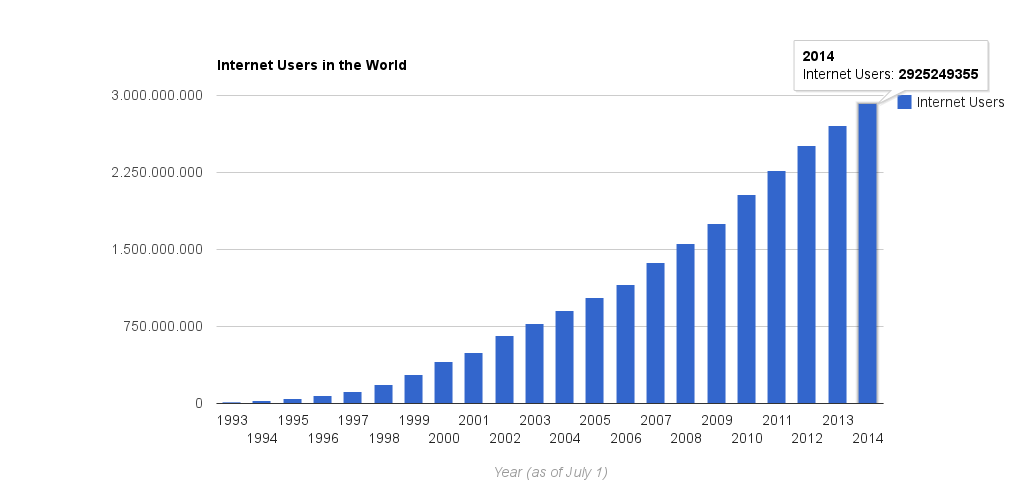
\includegraphics[scale=0.45]{images/internet_usage.png}
\caption{Quantidade de usuários da internet entre 1993 e 2014}
\label{fig:Quantidade de usuários da internet entre 1993 e 2014}
\end{figure}

\newpage

\item[Aplicações web] \hfill \\
A aplicação web refere-se a sistemas de informática que são executados através de navegadores com internet. Geralmente aplicações que utilizam-se de tecnologias web como HTML, Javascript e CSS.\cite{appWeb}

Quando é desenvolvida uma aplicação web que visa atender a este aumento significativo de acessos, surge-se a preocupação com a escalabilidade do sistema. Escalabilidade vem a ser ``a habilidade de uma aplicação manter o desempenho\footnote{Que significa ``a habilidade que uma aplicação tem de atingir um objetivo, como por exemplo responder no menor tempo possível'' \cite{escTerm}} quando a carga de trabalho aumenta'' \cite{escTerm}, podendo ser considerada uma junção entre capacidade\footnote{Que significa ``a carga total que uma aplicação pode suportar''\cite{escTerm}} e desempenho. 


\item[Escalabilidade em aplicações web] \hfill \\
Existem duas formas de escalabilidades, relacionadas as páginas web, a escalabilidade vertical e a horizontal.

Na escalabilidade vertical, há uma melhoria do hardware de um único servidor, quando é adicionada mais memória, ou o processador é trocado por outro mais potente, entre outros aspectos. 

A escalabilidade horizontal acontece quando são adicionados mais servidores, permitindo a criação de um \textit{cluster}\footnote{É um conjunto de computadores que subdividem o processamento do sistema para o aumento de desempenho, disponibilidade e balanceamento de carga.}. 

Estas duas formas de escalabilidade são geralmente relacionadas ao hardware, sendo utilizadas por páginas web que têm uma grande quantidade de acessos, e precisam continuar respondendo as requisições de maneira satisfatória\footnote{Por exemplo sem que o usuário perceba atrasos no carregamento da página}. 

Na figura \ref{fig: Escalabilidade vertical e horizontal}  pode-se observar de maneira mais clara a diferenciação entre escalabilidade vertical e horizontal.

\begin{figure}[htb]
\centering
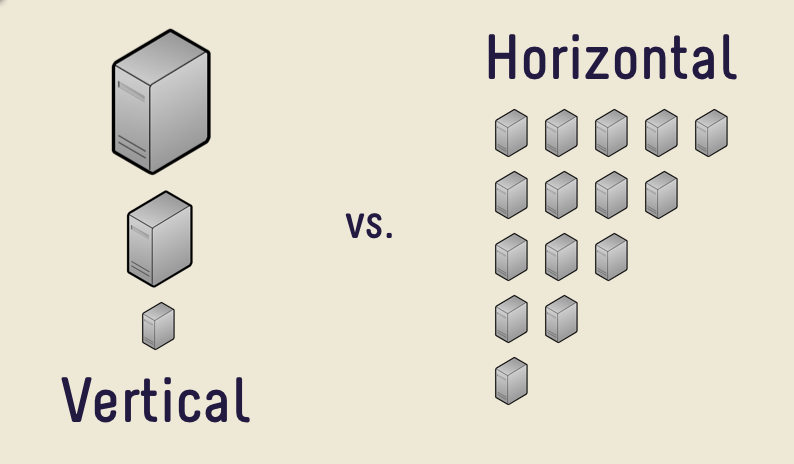
\includegraphics[scale=0.45]{images/scal_vh.png}
\caption{Escalabilidade vertical e horizontal \cite{ScalabVH}}
\label{fig: Escalabilidade vertical e horizontal}
\end{figure}

\newpage

Existem  situações em que a aquisição ou o melhoramento de servidores se torna algo muito custoso ou até mesmo inviável. Para essas situações são aplicadas técnicas de escalabilidade relacionadas ao software, que podem se subdividir em duas partes, que serão apresentadas a seguir:

\begin{itemize}
  \item A primeira é quando é realizado um simples acesso à página, ou seja, existem requisições do tipo \textit{http get}, neste caso para lidarmos com escalabilidade uma das soluções é a utilização de um proxy reverso\footnote{``Enquanto um proxy, no modelo convencional, intercepta requisições originadas na rede local (LAN – Local Área Network) com destino à Internet, um proxy reverso intercepta requisições originadas na Internet com destino à rede local.'' \cite{proxyRev}}, que pode funcionar como uma \textit{cache} para conteúdos estáticos\footnote{Musicas, imagens, vídeos, etc.} e dinâmicos\footnote{Que é quando um código é executado do lado do servidor para atender uma requisição, podendo realizar uma série de tarefas, como por exemplo acessar um banco de dados, sendo que este código é escrito em uma linguagem de programação como PHP, Java, Python, entre outras.}.

 \item A segunda parte é quando dados são enviados para serem persistidos através da página. Nesse caso estas requisições são do tipo \textit{http post}, e não há como efetuar \textit{cache} destes dados, pois são dados novos. As soluções encontradas nesse caso, são desde enfileirar as entradas para o banco de dados, até a utilização de banco de dados NoSQL.
\end{itemize}

\end{description}

\section{Programação orientada a eventos}
\label{sec:Programação orientada a eventos}
\nocite{eventDrivenPro}
A programação orientada a eventos ou programação dirigida a eventos é considerada um paradigma da programação\footnote{Um paradigma de programação fornece e determina a visão que o programador possui sobre a estruturação e execução do programa.} . A compreensão da orientação a eventos é importante para que se entenda algumas características do Node.JS. 

Entre outros paradigmas de programação pode-se citar \cite{prdgProg}:
\begin{itemize}
  \item Imperativa: é um paradigma de programação que descreve a computação como ações, enunciados ou comandos que mudam o estado (variáveis) de um programa.
  \item Estruturada: é uma forma de programação de computadores que preconiza que todos os programas possíveis podem ser reduzidos a apenas três estruturas: sequência, decisão e iteração (esta última também é chamada de repetição).
  \item Orientada a objetos: é um modelo de análise, projeto e programação de sistemas de software baseado na composição e interação entre diversas unidades de software chamadas de objetos.
  \item Funcional: é um paradigma de programação que trata a computação como uma avaliação de funções matemáticas e que evita estados ou dados mutáveis. Ela enfatiza a aplicação de funções, em contraste da programação imperativa, que enfatiza mudanças no estado do programa.
\end{itemize}

Um evento é qualquer ação do usuário que interaja com o sistema, por exemplo um clique do mouse em determinado local da aplicação, teclas do teclado sendo pressionadas ou até mesmo um toque na tela, caso o hardware permita como em smartphones e tablets modernos.

Um programa que utiliza orientação a eventos possui um fluxo que é um laço que recebe repetidamente informação para processar e disparam uma função de resposta de acordo com o evento recebido. As informações de entrada podem ser enfileiradas ou registrar uma interrupção, em alguns casos ambos podem ser adotados. Diferentemente do fluxo de linguagens tradicionais como C, onde o fluxo é linear com \textit{loops} no decorrer do caminho.

Para facilitar o entendimento imagine uma aplicação que mostra em sua tela o número zero. Esse número é incrementado ao se pressionar o botão esquerdo do mouse, decrementado ao se pressionar o botão direito do mouse, e volta para zero quando for pressionado o botão do meio. Esses cliques representam eventos, quando ocorrem, o sinal destes eventos são passados ao \textit{Event Loop}, que os trata e retorna o resultado. Nesse caso, o retorno é o incremento, decremento ou zerar o valor.

A figura \ref{fig:event loop} mostra como esse processo ocorre, destacando a interação dos eventos com o \textit{Event Loop}.

\begin{figure}[htb]
\centering
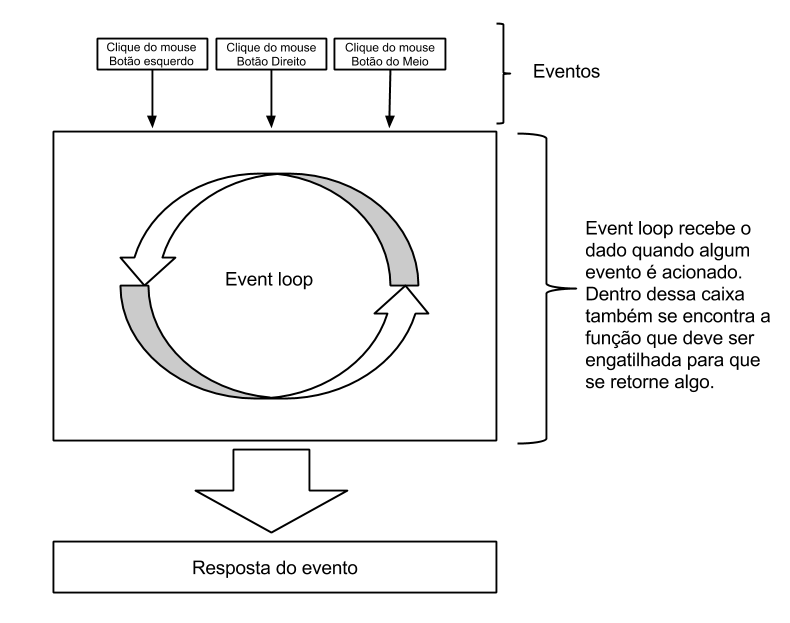
\includegraphics[scale=0.6]{images/event_loop_diagram.png}
\caption{Event Loop}
\label{fig:event loop}
\end{figure}

\newpage

\section{Javascript}
\label{sec: Javascript}
O Javascript  é uma linguagem de programação interpretada, que foi criada com o intuito de ajudar os navegadores web a executar scripts no lado do cliente e assim permitir a interação com o usuário\nocite{jsGood}. Esta linguagem foi baseada na ECMAScript\footnote{Que  é uma linguagem de programação de scripts.} que é padronizada pela Ecma international nas especificacões ECMA-262\footnote{\url{http://www.ecma-international.org/publications/files/ECMA-ST/Ecma-262.pdf}} e ISO/IEC 16262\footnote{\url{http://www.iso.org/iso/home/store/catalogue_tc/catalogue_detail.htm?csnumber=55755}}. Abaixo serão descritas algumas das principais características do Javascript:

\begin{description}
\item[Imperativa e estruturada] \hfill \\ 
O Javascript possui elementos de sintaxe de linguagens de programação estruturada, elementos que se assemelham por exemplo com a linguagem C como \textit{If}, \textit{while} e \textit{switch}.

Apesar de sintaticamente parecer com C, seu escopo é diferente, Javascript utiliza-se de um escopo a nível de função\footnote{Isso significa que somente funções podem criar novos escopos, blocos como \textit{if}, \textit{while}, \textit{for} não criam novos escopos.}.

\item[Tipagem dinâmica] \hfill \\
No Javascript os tipos são associados com valores e não com as variáveis. Por exemplo, uma variável ``A'' poderia ser associada a um número e posteriormente ser associada a uma string. 

% \item[Baseada em objetos] \hfill \\
% A linguagem Javascript possui suporte a  objetos, que são implementados como listas associativas. Os nomes das propriedades de um objeto  são strings e podem, junto com seus valores, ser adicionadas, mudadas ou apagada em tempo de execução. Vale ressaltar que em Javascript existem alguns objetos padrões como \textit{window} e \textit{document}.

\item[Baseada em protótipos] \hfill \\
 O Javascript utiliza-se de protótipos no lugar das classes para o mecanismo de herança. É possível simular muitas características de orientação a objetos usando-se protótipos.

\item[Linguagem orientada a eventos] \hfill \\
 No Javascript é possível tratar as interações do usuário em um arquivo HTML e é através de eventos que isso é feito, como explicado na seção \ref{sec:Programação orientada a eventos} deste capítulo .

\end{description}

\section{NoSQL - Not Only SQL}
\label{sec: NoSQL - Not Only SQL}
Os bancos de dados relacionais não foram desenvolvidos para resolver problemas enfrentados pelas aplicações web modernas como a escalabilidade e a agilidade \cite{mongoNosql}. ``Foram projetados para serem executados em uma máquina apenas'' \cite{compBds}. ``Quanto maior o tamanho, mais custoso se torna essa escalabilidade, seja pelo custo de novas máquinas, seja pelo aumento de especialistas nos bancos de dados utilizados''.\cite{IntNosql}

Devido às limitações citadas, começaram surgir diversas soluções que funcionam de maneira diferente aos tradicionais banco de dados relacionais. Essas soluções ficaram conhecidas como NoSQL - \textit{Not Only SQL}. Pode-se categoriza em ``uma nova classe de banco de dados'' \cite{AnaliseNosql}, formada por ``diferentes sistemas de armazenamento ''\cite{NosqlIm}, que surgiu para lidar com situações em que os bancos de dados tradicionais são ineficientes. ``Muitas dessas bases apresentam características muito interessantes como alta performance, escalabilidade, replicação, suporte à dados estruturados e sub colunas''\cite{NosqlIm}. 

Seguem abaixo algumas características de bancos de dados NoSQL\cite{compBds}:
\begin{itemize}
\item Não usa modelo de dados relacional e portanto não usa a linguagem SQL;
\item Costuma ser projetado para ser executado em um \textit{cluster};
\item Costuma ser \textit{open-source};
\item Não possui esquema fixo (\textit{SCHEMA-LESS}), permitindo gravar qualquer dado em qualquer estrutura.
\end{itemize}

Existem diversas categorias\cite{NosqlDatabase} em que se classificam os banco de dados NoSQL que variam de acordo com a forma de armazenar os dados. Algumas das  principais categorias que se destacam são: chave/valor, orientado a colunas, orientado a documentos e baseado em grafos \cite{AnaliseNosql}.
\begin{description}
\item[Chave/Valor] \hfill \\ 
Utiliza um \textit{array} associativo como modelo de dados \cite{NosqlWiki}. Nestes \textit{array} os dados podem ser acessados através de chaves, e estas chaves estão associadas a seus valores correspondentes. Alguns bancos desta categoria são: Azure Table Storage, Berkeley DB,Couchbase, DynamoDB, Redis, Riak e Tokyo Cabinet.

%exemplos
\item[Orientado a colunas] \hfill \\ 
Em um banco de dados orientado a colunas ``ao invés de cada registro da tabela ficar armazenado em uma linha, o registro passa a ser armazenado em colunas separadas.''\cite{NosqlCol}. Como exemplo de banco de dados desta categoria são:  Hadoop, Cassanda, Hypertable e Amazon SimpleDB.

% Essa forma de armazenamento tem algumas vantagens, como exemplo a capacidade de compressão dos dados, se formos analisar a compressão de um banco onde os registros são armazenados em linha, encontraremos em uma mesma linha diferentes tipos (domínios) o que torna o processo mais complicado, já no banco orientado a colunas, cada coluna irá conter o mesmo tipo (domínio) de dado. De acordo com algumas pesquisas o nível de compressão alcançado  em bancos orientados a colunas chega a ser de 60% a 70%  mais eficiente que nos bancos orientados a linhas.
\item[Orientado a documentos] \hfill \\ 
Nesta categoria de banco de dados, o armazenamento é realizado através de documentos, e o conjunto de documentos forma uma coleção. Geralmente os documentos são codificados nos formatos JSON, XML e YAML\cite{NosqlWiki}. Alguns dos bancos de dados que pertencem a esta categoria são: MongoDB, CouchDB e EjDB.


\item[Baseado em grafos] \hfill \\ 
Quando se tem dados cujas relações são bem representadas como um grafo, pode se  utilizar um banco de dados baseado em grafos \cite{NosqlWiki}. Com este modelo é possível ``representar os dados e/ou o esquema dos dados como grafos dirigidos ou como estruturas que generalizem a noção de grafos.'' \cite{IntNosql}

Alguns bancos que fazem parte desta categoria são: Neo4J, Infinite Graph, Titan, e Bigdata.

\end{description}

%\section{Vantagens da utilização do MEAN para o desenvolvimento de aplicações escaláveis}


\chapter{Tecnologias}
\label{tecnologias}
Este capítulo tem como foco explicar cada uma das tecnologias propostas neste texto, abordando algumas particularidades que servem para resolver o problema de escalabilidade. 

Primeiramente na seção \ref{sec: MEAN} será explicado o conceito da sigla MEAN, e as subseções seguintes detalharão cada uma das tecnologias propostas. Na subseção \ref{subsec: MongoDB} será explicado o MongoDB. Na subseção \ref{subsec: Express.js} será apresentado o Express.js. Na subseção \ref{subsec: AngularJS} aborda-se sobre o AngulaJS. Na subseção \ref{subsec: Node.js} o foco será no Node.js. 

\section{MEAN \textit{Stack}}
\label{sec: MEAN}
O nome MEAN é um acrônimo que representa o conjunto de quatro ferramentas:
o banco de dados NoSQL \textbf{M}ongoDB\footnote{http://www.mongodb.org/}, o \textit{framework back-end} \textbf{E}xpress\footnote{http://expressjs.com/} , o framework front-end \textbf{A}ngularJS\footnote{https://angularjs.org/}, e o servidor \textbf{N}odeJS\footnote{http://nodejs.org/}. O MEAN foi concebido através de um debate de usuários em um grupo no Linkedin\footnote{https://www.linkedin.com/groups/Mean-Stack-5070069}. Nos subtópicos abaixo serão abordadas as principais características de cada uma dessas ferramentas.

\subsection{MongoDB}
\label{subsec: MongoDB}
O MongoDB é um banco de dados de código aberto do tipo NoSQL. Foi implementado na linguagem  C++ e é orientado a documentos. O formato dos documentos utilizados pelo MongoDB é o JSON\footnote{\textit{JavaScript Object Notation}, é um formato de texto baseado no conceito de chave-valor, que serve para troca de informações/dados entre sistemas.}/BSON\footnote{Internamente este formato é convertido para BSON, que é um arquivo JSON no formato binário, que foi criado para tornar mais eficiente a busca e o espaço de armazenamento.}. Utiliza-se este formato pela facilidade na integração de dados em certos tipos de aplicações. O nome Mongo vem da expressão da língua inglesa ``humongous'',  que significa ``monstruoso'' ou ``gigantesco''. 

Algumas razões por optarem pelo Mongo para funcionar junto com ferramentas Javascript são: o tratamento de objetos JSON,  possuir uma boa aceitação por parte da comunidade de desenvolvedores\cite{dbEng}, ter um bom desempenho com grande volume de dados \cite{compBds}, a capacidade de executar códigos em Javascript  para as consultas, além de possuir uma grande integração\footnote{Através do próprios drives, e com a utilização da api Mongoose.} com Node.js.   

A tabela \ref{fig:Tabela comparando as terminologias do SQL e do MongoDB} apresenta várias terminologias e conceitos padrões do SQL e as terminologias e conceitos correspondentes que o MongoDB utiliza.

\begin{table}[ht]
\begin{tabular}{|l|l|}
\hline
\rowcolor[HTML]{CFCFCF} 
Termos/Conceitos SQL & Termos/Conceitos MongoDB \\ \hline
base de dados        & base de dados          \\ \hline
tabela               & coleção                \\ \hline
linha                & documento (BSON)       \\ \hline
coluna               & campo                  \\ \hline
índice               & índice                 \\ \hline
joins                & documentos incorporados (\textit{embedded})                                            \\ \hline
chave primária       & chave primária         \\ \hline
                     &                        \\
\multirow{-2}{19em}{Especificar uma coluna ou um conjunto   de colunas como chave primária} & \multirow{-2}{19em}{No MongoDB, a chave primária é  automaticamente atribuída ao campo \_id} \\ \hline
\end{tabular}
\caption{Comparação entre as terminologias do SQL e do MongoDB. \cite{MongoDbSQL}}
\label{fig:Tabela comparando as terminologias do SQL e do MongoDB}
\end{table}

% \begin{figure}[!ht]
% \centering
% 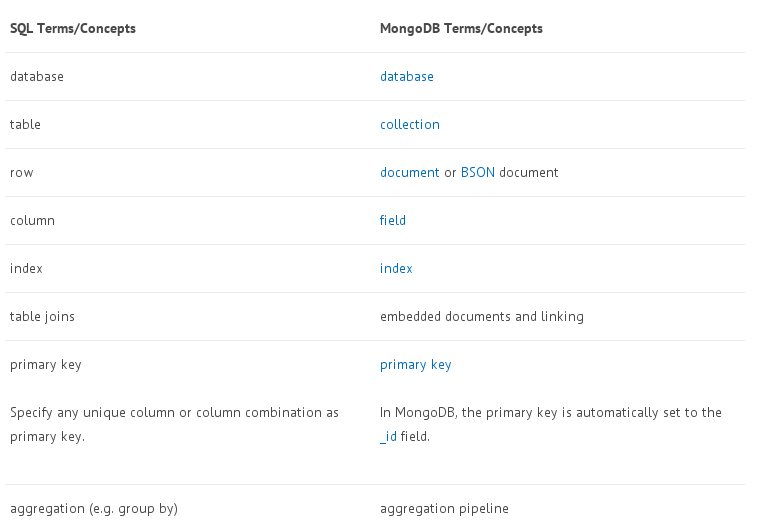
\includegraphics[scale=0.7]{images/comp_mongo_sql.png}
% \caption{Gráfico comparando as terminologias do SQL e do MongoDB.}
% \label{fig:Gráfico comparando as terminologias do SQL e do MongoDB}
% \end{figure}

\begin{description}
\item[Escalabilidade através do Sharding] \hfill \\ 
 O termo \textit{Sharding} é uma técnica de escalabilidade horizontal em que os dados de uma base de dados são divididos em muitos \textit{Shards}, os quais podem ser distribuídos entre várias máquinas \cite{AnalysisNoSQL}.

O MongoDB tem suporte a uma técnica conhecida como \textit{Autosharding}, que ``permite a construção de um \textit{cluster} de banco de dados escalável horizontalmente projetado para incorporar novas máquinas de forma dinâmica'' \cite{BdNoSQLxSGBDs}.

O \textit{cluster} é formado de três componentes: blocos de servidores chamados \textit{Shards}, que são reponsáveis pelo armazenamento dos dados, os servidores de configuração chamados de \textit{mongod}, que contêm os metadados e as informações de rotas, e os serviço de rotas chamados \textit{mongos}, que são responsáveis ``pelo roteamento das operações ao destino apropriado''\cite{BdNoSQLxSGBDs}.

A figura \ref{fig: Topologia do Sharding}  abaixo mostra como os componentes que constituem o \textit{cluster} do MongoDB interagem para prover uma escalabilidade horizontal.  
\begin{figure}[!ht]
\centering
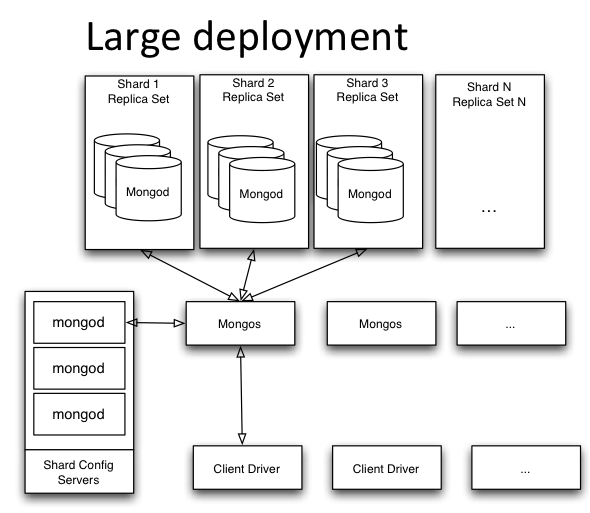
\includegraphics[scale=0.7]{images/1sharding_topology.png}
\caption{Topologia do Sharding. \cite{MongoPy}}
\label{fig: Topologia do Sharding}
\end{figure}

\item[Armazenamento] \hfill \\
O MongoDB ``mapeia diretamente um arquivo armazenado em disco para um array de bytes em memória virtual, não memória física RAM, onde a lógica de acesso aos dados é implementado usando aritmética de ponteiro. O uso de arquivos mapeados em memória é eficiente para melhorar o desempenho''\cite{AnaliseNosql}.

Uma das características do MongoDB é a de ter consistência eventual (\textit{eventual consistency}), que significa que  existe um momento apropriado para o sistema tornar-se consistente. \cite{BaseAcid}

O gerenciador de memória virtual do sistema operacional é responsável por decidir quais partes da base de dados vão para o disco e quais ficam em memória. Este mecanismo faz com que o MongoDB não tenha controle sobre quando os dados são escritos no disco\cite{AnalysisNoSQL}.

\end{description}


\subsection{Express.js}
\label{subsec: Express.js}
O Express.js é um \textit{framework} que visa facilitar o desenvolvimento de aplicações Web com o Node.js. O Express.js permite criar servidores web e receber requisições HTTP de maneira simples. Ele também permite a criação de um conjunto de diretórios com uma estrutura padrão, além de organizar as rotas dos arquivos para as \textit{views} da aplicação. Geralmente os projetos que utilizam-se do Express também aderem a algum \textit{framework} de \textit{templates} como Jade ou EJS.

\subsection{AngularJS}
\label{subsec: AngularJS}
AngularJS é um \textit{framework} javascript \textit{client-side} que segue o modelo MVC\footnote{MVC (\textit{Model-View-Controller}, que em português é Modelo-Visão-Controlador) é uma forma de estrutura seu projeto/aplicação de forma que a interface de interação (\textit{views}) esteja separada do controle da informação em si (\textit{models}), separação essa que é intermediada por uma outra camada controladora (\textit{controllers}).} e é mantido pela Google.

Existem muitos outros frameworks além do AngularJS, e ao meio de tanta competitividade ele tem se destacado. O gráfico apresentado na figura \ref{fig:Gráfico Comparando Frameworks Javascript} é um bom argumento para mostrar a popularidade do AngularJS.

A figura \ref{fig:Gráfico Comparando Frameworks Javascript} foi retirada do site ``Info Q \cite{fwJs}'', onde foi realizado uma enquete para saber qual \textit{framework} é mais utilizado pelos desenvolvedores. A enquete é realizada como um \textit{drag and drop}, onde o usuário que está votando terá que posicionar o nome da aplicação entre os dois eixos do gráfico de acordo com sua opinião.

A linha vertical, \textit{``Value Proposition''}, representa a importância da aplicação para o usuário que está votando, a linha horizontal, \textit{``Adoption Readiness''} representa o quanto o usuário usa a aplicação na vida real. 

O tamanho dos circulos do gráfico represetam a quantidade de votos recebidos.

\begin{figure}[!ht]
\centering
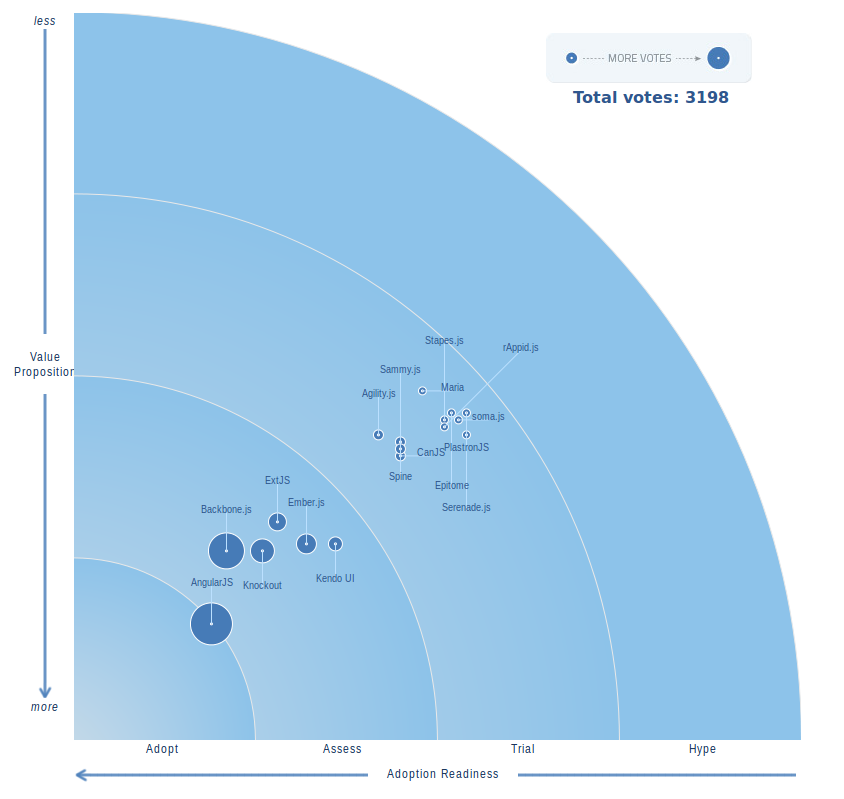
\includegraphics[scale=0.5]{images/angularjs_framework_comparison.png}
\caption{Gráfico comparando frameworks Javascript. \cite{fwJs}}
\label{fig:Gráfico Comparando Frameworks Javascript}
\end{figure}

\newpage

Algumas características que se destacam no AngularJS são:
\begin{description}
\item[SPA - \textit{Single Page Application}] \hfill \\ 
O conceito de Single Page Application é que cada parte de página é carregada de forma independente, ou seja, quando uma página é carregada, todas as demais atualizações são feitas através de requisições AJAX\footnote{AJAX é uma metodologia que utiliza tecnologias como XML e Javascript para fazer requisições assíncronas ao servidor e com as informações retornadas modificar uma página carregada através do DOM, sem a necessidade de recarregar todo seu conteúdo.} e renderizações parciais na página.

    Através destas renderizações parciais tem-se um aumento de desempenho devido à diminuição da quantidade de dados que precisam ser trafegadas entre o cliente e o servidor.

\item[\textit{Two-Way Data Biding}] \hfill \\
É um mecanismo para facilitar o desenvolvimento do sistema, pois reduz a quantidade de código escrito.
\textit{Two-way Data biding} funciona por meio de processo que sincroniza os dados na \textit{view} e no \textit{model} como aparesentado na figura \ref{fig:Two-way databiding}. 

\begin{figure}[htb]
\centering
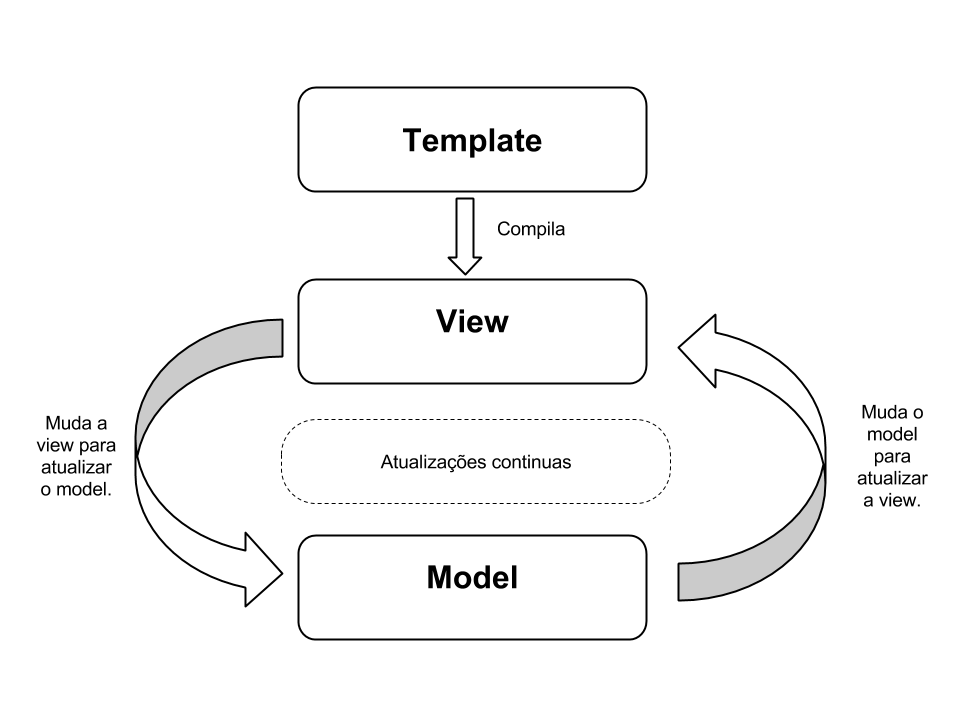
\includegraphics[scale=0.35]{images/Two_way_databiding_diagram.png}
\caption{Digrama do \textit{Two-way data biding} \cite{TwoWayData}}
\label{fig:Two-way databiding}
\end{figure}

\newpage

\item[Injeção de dependências] \hfill \\
A injeção de dependências consiste basicamente  em fornecer recursos extras necessários na aplicação de forma transparente ao usuário, de modo que o desenvolvedor somente deverá solicitar um recurso, que será injetado pelo \textit{framework} e ficará disponível para uso.
\end{description}

\subsection{Node.js}
\label{subsec: Node.js}
\nocite{poeNode}
\nocite{MongoNode}
O Node.js é uma plataforma de desenvolvimento web que funciona com a linguagem Javascript no lado do servidor, para criação de aplicações e páginas web de alta escalabilidade. 

Foi concebida por  Ryan Dahl em 2009 \nocite{appRealTime}, e desde então vem ganhando muita popularidade entre os desenvolvedores web, e sendo utilizado por grandes empresas e instituições tais como LinkedIn, Microsoft, GitHub, MySpace, entre outras\cite{compNode}.

A escolha da linguagem Javascript foi devido a enorme quantidade de bibliotecas para I/O que a linguagem possui, permitindo assim criar as funções assíncronas para a plataforma.

A arquitetura do Node.js é composta em sua maior parte por componentes  desenvolvidos em C e em Javascript \nocite{nodeInAction}. Os principais componentes da parte escrita em C são: a \textit{V8 Javascript Engine}\footnote{É máquina virtual para Javascript do Google utilizada no navegador Chrome, que ``compila e executa código fonte JavaScript, lida com a alocação de memória para objetos e limpa-os quando não são mais necessários''\cite{v8Eng}.}, o \textit{Node Bindings}\footnote{São códigos executáveis que fazem com que o V8 e a biblioteca em javascript padrão do node sejam capazes de se comunicar.}, a  \textit{Thread Pool}\footnote{``É uma coleção de \textit{threads} disponíveis para realizar tarefas''\cite{ThreadPool}}, e o \textit{Event Loop}. Para a parte responsável pelo Javascript, foi criada uma biblioteca chamada \textit{Node Standard Library}, para permitir que o Node.js interprete códigos em Javascript.

Abaixo segue a figura \ref{fig:Arquitetura do Node.js} que concede um modelo visual desta arquitetura, com o intuito de facilitar o entendimento da relação entre os componentes citados do Node.js.

\begin{figure}[htb]
\centering
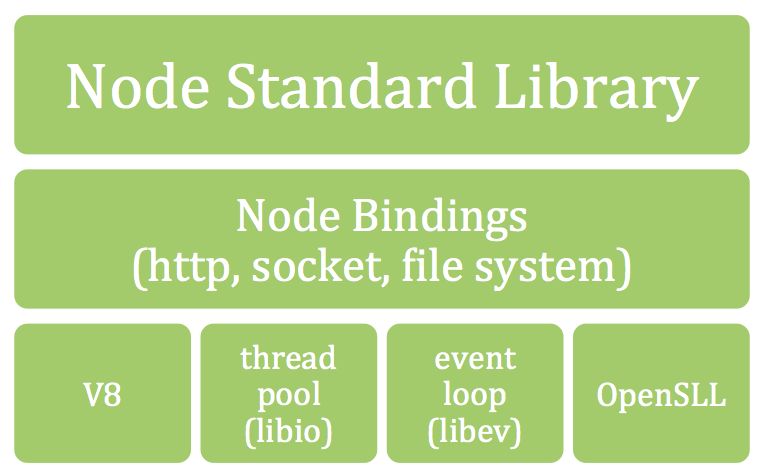
\includegraphics[scale=0.4]{images/node_platform.png}
\caption{Arquitetura do Node.js. \cite{nodeMeet}}
\label{fig:Arquitetura do Node.js}
\end{figure}
    
    O Node.js foi criado de forma que suas funcionalidades pudessem ser estendidas através de módulos, para implementar diversos componentes \textit{middleware} que facilitem o desenvolvimento de aplicações web. Estes módulos são geralmente instalados através de um gerenciador de pacotes conhecido como npm, que significa \textit{Node Package Manager}, e serve para facilitar diversos aspectos relacionados à aplicação como a compilação, a instalação e a atualização e também funciona como um gerenciador de dependências.

\begin{description}
\item[I/O não bloqueante e orientado a eventos] \hfill \\
Quando é necessario acessar\footnote{Seja para leitura, escrita, atualização ou remoção.} os dados de uma aplicação, estes dados podem estar em vários locais, tais como na memória (L1, L2, RAM), no disco ou na rede. Cada local contém uma latência de I/O diferente, no caso para memória quando se necessita acessar a L1 é gasto aproximadamente  3 ciclos, passando para 14 ciclos na L2 e para 250 ciclos na RAM. Já para o disco e para a rede a quantidade de ciclos necessários tem um aumento significativo, sendo aproximadamente 41 e 250 milhões de ciclos, respectivamente. Ou seja, quando utiliza-se a memória é possível considerar que será um acesso rápido, também conhecido como não bloqueante, enquanto para o disco e a rede considera-se que será um acesso lento, também conhecido como bloqueante.

A figura \ref{fig:Event Loop do Node.js} demonstra como é o funcionamento do \textit{Event Loop} no Node.js, que tem como entrada uma fila (\textit{queue}) de requisições, e no caso de ser recebido uma requisição bloqueante, esta requisição é passada para uma \textit{Thread Pool}, que irá tratar o evento, caso contrário o evento é tratado no próprio \textit{Event Loop}.

\begin{figure}[ht]
\centering
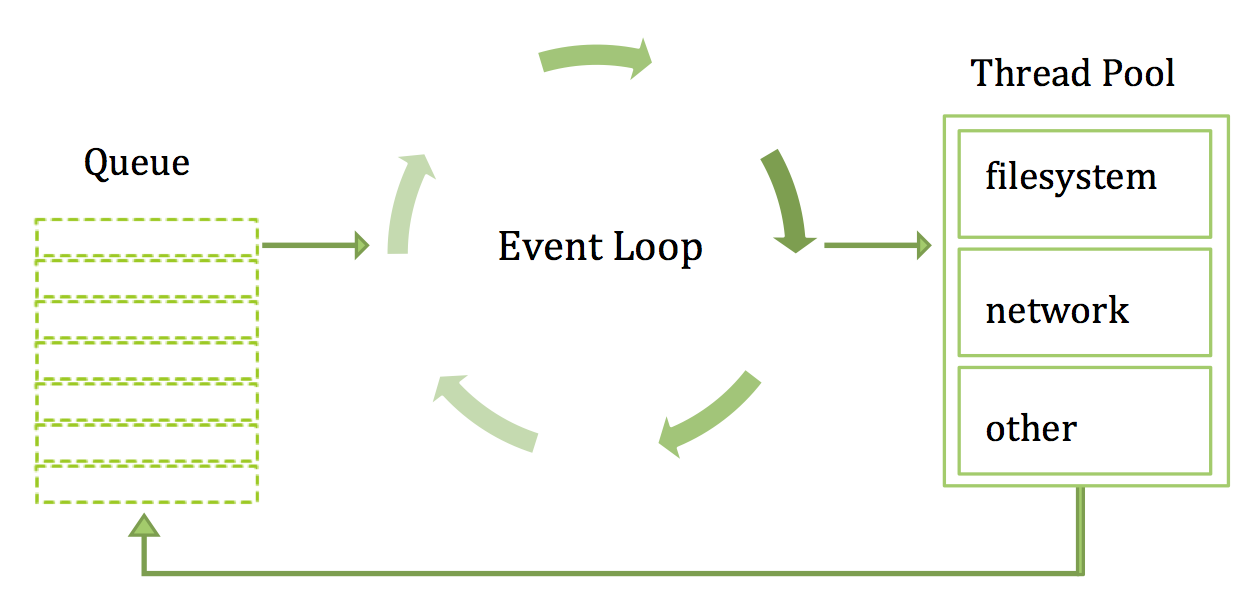
\includegraphics[scale=0.3]{images/node_event_loop.png}
\caption{Event Loop do Node.js. \cite{nodeMeet}}
\label{fig:Event Loop do Node.js}
\end{figure}

O Node.js foi desenvolvido com base no conceito de ``I/O não bloqueante''\nocite{nodeRight}  (também conhecido por I/O assíncrono), e isto foi feito através da utilização e adaptação de uma construção  de programação conhecida como \textit{Event Loop}, que foi apresentado na seção \ref{sec:Programação orientada a eventos} do capítulo \ref{cha: Conceituação e Idéia Geral}.

A execução do Node.js geralmente funciona através de uma única \textit{thread} e quando existe a necessidade de I/O bloqueante, uma \textit{thread} pertencente à \textit{Thread Pool} fica responsável por lidar com este tipo de I/O.  

Um exemplo do funcionamento do \textit{Event Loop} do Node.js é quando se recebe uma requisição de um evento não bloqueante, sendo que este evento será tratado diretamente pela \textit{thread} principal. Outra situação é quando se recebe uma requisição bloqueante, por exemplo uma leitura de disco, esta requisição então é enviada para a \textit{Thread Pool} do Node.js. A \textit{Thread Pool} irá utilizar uma \textit{thread} para tratá-la, e quando terminar, a \textit{thread} responsável pelo processamento bloqueante envia uma mensagem para a \textit{thread} principal, que então executa a função de \textit{callback}\footnote{''é um mecanismo de controle de fluxo que visa beneficiar processos assíncronos.''\cite{StackOCallbk}} respectiva à requisição.
    
\end{description}


\chapter{Aplicações web com MEAN \textit{Stack}}	 
\label{implementacao}

%\section{Aplicação Math Race  desenvolvido com outras tecnologias}

    No capitulo três foi apresentado cada elemento do MEAN \textit{Stack} individualmente. Neste capítulo será apresentado e analisado, como estes elementos funcionam em conjunto, formando uma pilha (\textit{Stack}).

Na seção \ref{Comparativo em relação a arquitetura de aplicações LAMP} é apresentado um comparativo entre o MEAN \textit{Stack} e a arquitetura LAMP. A integração das ferramentas do MEAN \textit{Stack} é apresentada na seção \ref{Aplicação Math Race com MEAN Stack}. Na seção \ref{subsec: Testes de desempenho}  são  mostrados os testes realizados em relação ao desempenho.

A figura \ref{fig:MEAN Stack visto como uma pilha} ilustra a pilha que é formada unindo as tecnologias já explicadas no capítulo anterior. No banco de dados coloca-se o MongoDB, no lado do servidor existe o Node.js e o Express e por último no lado do cliente o AngularJS. A seta de duplo sentido representa que a passagem de dados acontece em ambos os sentidos. O principal motivo para estas tecnologias funcionarem bem em conjunto, é que todas elas têm como base a linguagem Javascript, sendo que esta característica faz parte da proposta do MEAN \textit{Stack} que é o desenvolvimento de aplicações web escaláveis com a utilização de um conjunto de ferramentas em Javascript.
    
\begin{figure}[htb]
\centering
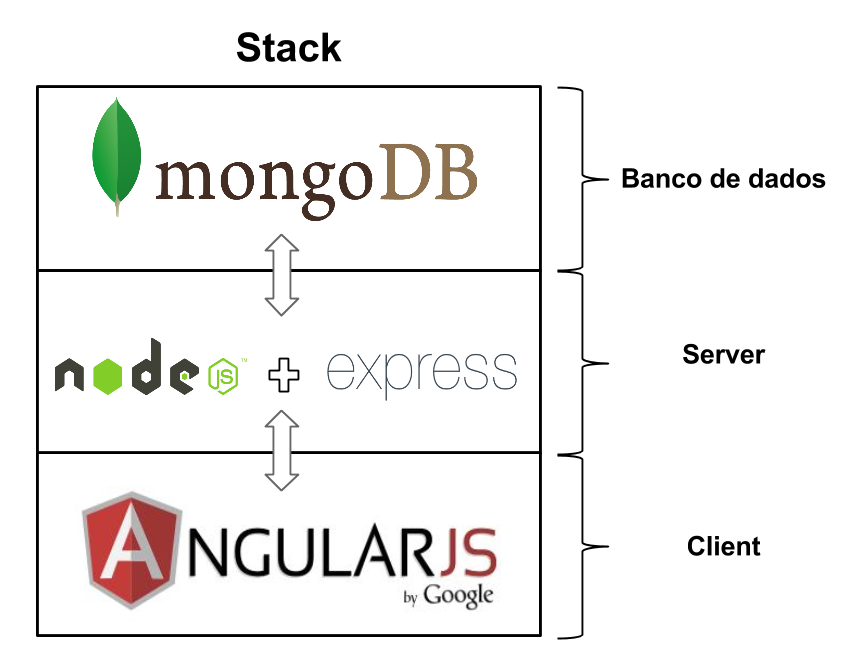
\includegraphics[scale=0.4]{images/mean_stack_diagram.png}
\caption{MEAN \textit{Stack} visto como uma pilha}
\label{fig:MEAN Stack visto como uma pilha}
\end{figure}

\newpage   
  
\section{Comparativo em relação ã arquitetura de aplicações LAMP}
\label{Comparativo em relação a arquitetura de aplicações LAMP}
    Para cada componente da pilha existe uma quantidade razoável de tecnologias semelhantes. Se for utilizada  como exemplo a figura \ref{fig:Gráfico Comparando Frameworks Javascript}, mostrada no capítulo \ref{tecnologias}, pode-se observar uma grande quantidade de tecnologias concorrentes que existem, cada uma se destacando em alguma situação. Neste cenário torna-se muito complicado concluir o que é melhor, ainda mais que o próprio MEAN pode variar, por exemplo para PEAN quando o MongoDB é substituído pelo PostgreSQL. 
    A comparação do MEAN será feita com o LAMP, pois este tem um destaque quando o assunto se trata de aplicações web. \cite{meanVSlamp}
   
   Assim como o MEAN, o LAMP é uma pilha de software livres com o foco no desenvolvimento web. A sigla LAMP é um acrônimo de Linux, Apache, MySQL e Perl/PHP/Python.
   
   Uma característica que difere os dois conjuntos de ferramentas, é que o LAMP necessita do Linux ou outro sistema operacional, ficando dependente do sistema escolhido. Enquanto o MEAN pode ser executado em qualquer plataforma.
   
    O servidor do MEAN é o Node.js, enquanto ao do LAMP é Apache. O que destaca o Node.js neste caso é o fato de ser totalmente não bloqueante e ser orientado a eventos, como já citado na subseção 3.1.4, o que permite concorrência entre as requisições. Porém como o Node.js é recente, não existe muitos \textit{plugins} que auxiliam seu uso, o que não acontece com o Apache, que já está há muito tempo no mercado, sem dizer que em muitos casos ele é escolhido como servidor padrão de muitos desenvolvedores.
    
    O Banco de dados do MEAN é o MongoDB, que como já explicado anteriormente pertence a categoria NoSQL. O LAMP utiliza o MySQL, que pertence a categoria SQL. Para comparação entre esses bancos de dados deve-se considerar a situação, por exemplo uma consulta com intuito de retornar um valor no MongoDB é mais rápida do que no MySQL, pois o MongDB não possui \textit{schemas} de tabelas mas sim um arquivo \textit{JSON}. Em contrapartida, a atualização dos dados do banco pode ser muito lenta para o MongoDB, isso considerando que existem muitos dados armazenados no banco.
    
    Para o desenvolvimento da aplicação no lado do cliente, o MEAN e o LAMP seguem abordagens consideravelmente diferentes, enquanto no MEAN \textit{Stack} a ferramenta responsável é o AngularJS, no LAMP não há uma ferramenta padrão definida.  
    
    No lado do servidor, o MEAN \textit{Stack} utiliza o  Express.js e o Node.js, e o LAMP, pode ser codificado através de três linguagens de programação: Perl, PHP ou Python.
    
    No MEAN, o Express.js serve como a camada de controle, empacotando os dados e enviando para AngularJS que utiliza a informação para realizar alguma ação e renderizar a página. A principal vantagem de se utilizar o AngularJS é que ele funciona totalmente no lado do cliente, como já foi explicado no capítulo anterior.
    
    Todas as características citadas nesta seção podem ser observadas, de forma mais direta, na tabela \ref{fig:tabela mean vs lamp}.
    
    O fato de todas as tecnologias do MEAN serem em Javascript, garante que o desenvolvedor precise saber apenas uma linguagem de programação. Porém isso também tem seu lado negativo, que é o engessamento do projeto só em Javascript, ou seja seu projeto fica dependente apenas do que o Javascript consegue fazer.
    
    % \begin{figure}[htb]
    % \centering
    % 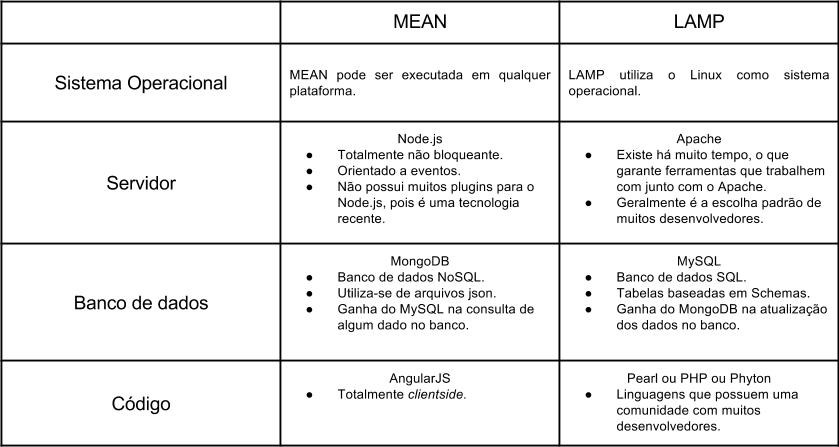
\includegraphics[scale=0.5]{images/mean_vs_lamp.png}
    % \caption{Tabela de comparação entre MEAN vs LAMP}
    % \label{fig:tabela mean vs lamp}
    % \end{figure}

\begin{table}[ht]
\centering
\begin{tabular}{|p{4cm}|p{5cm}|p{5cm}|}
\hline
\rowcolor[HTML]{CFCFCF} 
    & MEAN                                                                                                                   & LAMP                                                                                                                   \\ \hline
    Sistema Operacional & Pode ser executada em qualquer plataforma. & Utiliza o Linux como sistema operacional. \\ \hline
    Servidor 
    
    & \textbf{Node.js} 
    
    - Totalmente não bloqueante. 
    
    - Orientado a eventos. 
    
    - Não possui muitos plugins para o Node.js, pois é uma tecnologia recente. 
    
    & \textbf{Apache}
    
    - Existe há muito tempo, o que garante ferramentas que trabalhem com junto com o Apache. 
    
    - Geralmente é a escolha padrão de muitos desenvolvedores. \\ \hline
    Banco de dados & \textbf{MongoDB} 
    
    - Banco de dados NoSQL. 
    
    - Utiliza-se de arquivos JSON. 
    
    - Ganha do MySQL na operação de consulta no banco de dados. 
    
    & \textbf{MySQL} 
    
    - Banco de dados SQL. 
    
    - Tabelas baseadas em \textit{Schemas}. 
    
    - Ganha do MongoDB na atualização dos dados no banco. \\ \hline
    
    Codificação & \textbf{AngularJS}
    
    - No lado do cliente. 
   
    \textbf{Express.js} e \textbf{Node.js} 
    
    - No lado do servidor & \textbf{Pearl}, \textbf{PHP} ou \textbf{Phyton} 
    
    - No lado do servidor.  
    
    - Possuem uma comunidade com muitos desenvolvedores.  \\ \hline
\end{tabular}
\caption{Tabela de comparação entre MEAN vs LAMP}
\label{fig:tabela mean vs lamp}
\end{table}

\newpage
   
\section{Aplicação \textit{Math Race} com MEAN \textit{Stack}}
\label{Aplicação Math Race com MEAN Stack}
Nesta seção será apresentada uma aplicação desenvolvida com o MEAN \textit{Stack}. A subseção \ref{subsec: Proposta de desenvolvimento} descreve a proposta de desenvolvimento da aplicação. A subseção \ref{subsec: Utilização e funcionamento da aplicação} mostra como é a utilização e o funcionamento da aplicação. A subseção \ref{subsec: Desenvolvimento da aplicação} aborda como foi desenvolvida a aplicação. 

\subsection{Proposta da aplicação}
\label{subsec: Proposta de desenvolvimento}
 Uma aplicação simples foi desenvolvida, com o intuito de demonstrar diversos aspectos do MEAN \textit{Stack}, como a organização e a integração das ferramentas que compõem o MEAN \textit{Stack}. A aplicação foi baseada na implententação do \textit{Math Race}, desenvolvida por Iván Loire\cite{MathRace}, possuindo apenas o Node.js e o Socket.io como ferramentas em comum.

\subsection{Utilização e funcionamento da aplicação}
\label{subsec: Utilização e funcionamento da aplicação}
 A aplicação é um jogo, cujo objetivo é realizar uma competição em tempo real, para ver qual jogador acerta mais operações de matemáticas aleatórias de adição e subtração, em determinado tempo.

Na figura \ref{fig:Imagem da interface da aplicação} é mostrada a interface da aplicação, que contém a operação aleatória, o campo para entrada de dados, o marcador de tempo (\textit{Time}), o campo de pontuação (\textit{score}) e o Hall da fama (\textit{Hall of fame}).

    \begin{figure}[htb]
    \centering
    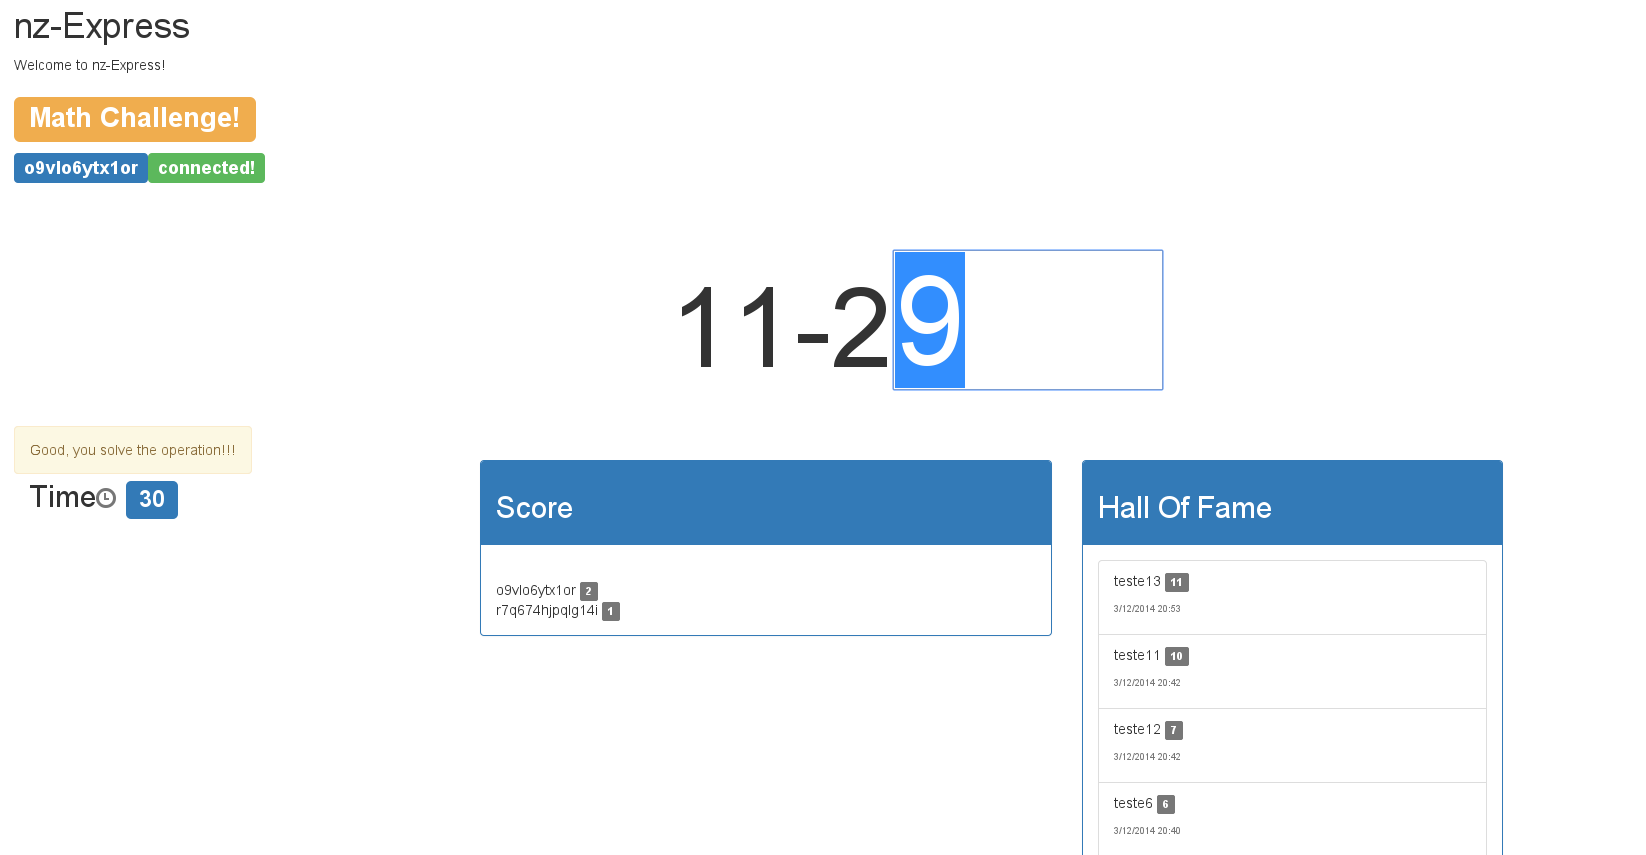
\includegraphics[scale=0.3]{images/index_mean_math_race.png}
    \caption{Imagem da interface da aplicação}
    \label{fig:Imagem da interface da aplicação}
    \end{figure}
    
Todos os jogadores possuem o mesmo tempo para responder a mesma operação matemática. A operação matemática muda para todos os jogadores após a resposta correta da operação anterior ter sido preenchida por qualquer jogador.

O jogo funciona através de rodadas, e para cada rodada o usuário tem um tempo limite pré-determinado para acertar o resultado da conta. A cada resultado correto o valor da pontuação do usuário, que começa em zero, é incrementado com mais um ponto. Ao final de uma rodada os usuários que efetuaram alguma pontuação são adicionados no ``Hall da fama'', que é ordenado pelos dez usuários com mais pontos obtidos em uma única rodada, e as pontuações dos usuários são zeradas, para que uma nova rodada se inicie. 

Na figura \ref{fig: Diagrama do funcionamento da aplicação} é demonstrado, através de um diagrama, o funcionameto da aplicação. 

    \begin{figure}[htb]
    \centering
    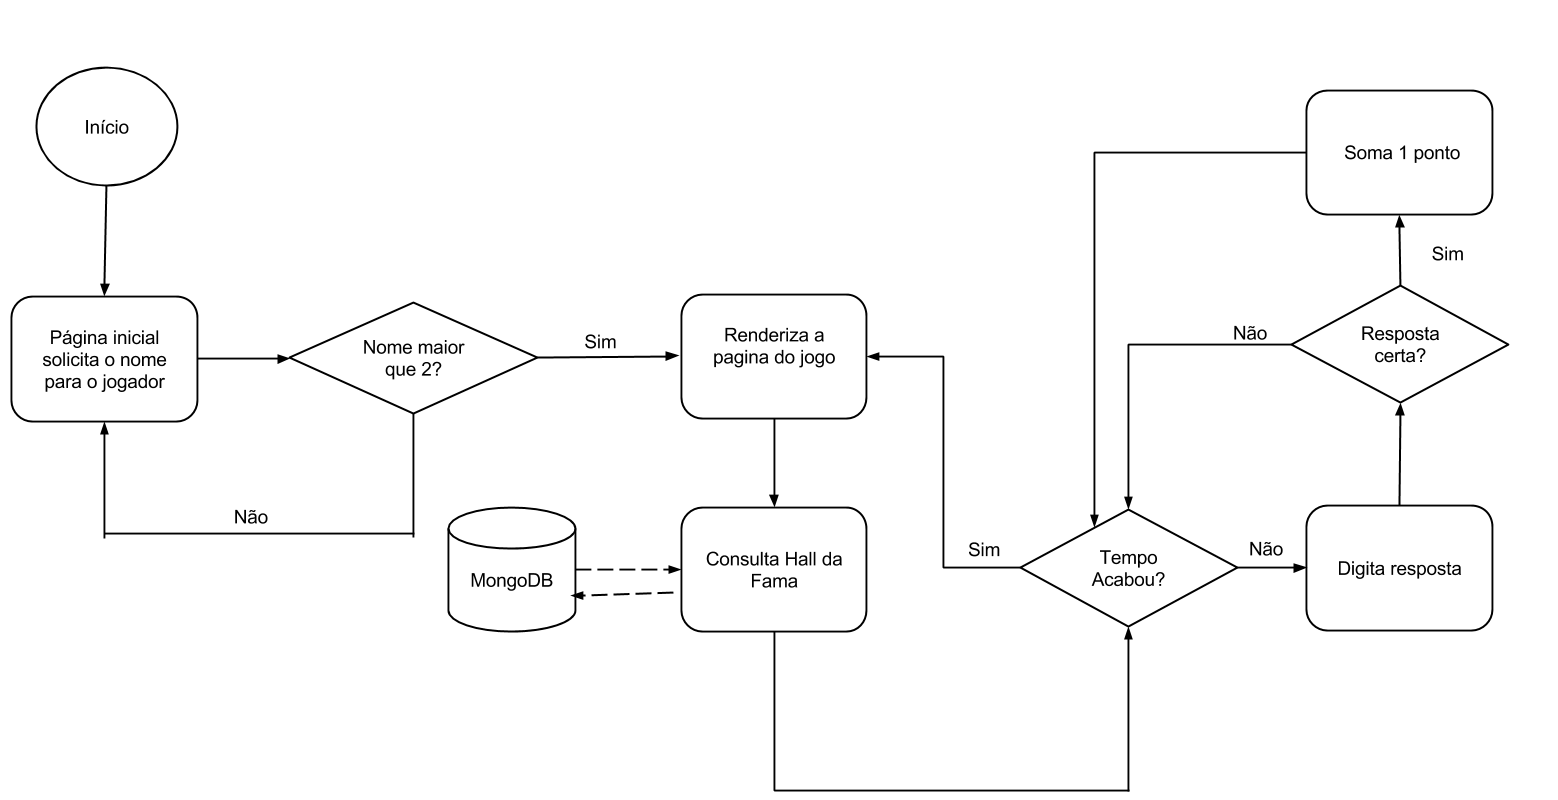
\includegraphics[scale=0.30]{images/func_mr.png}
    \caption{Diagrama do funcionamento da aplicação}
    \label{fig: Diagrama do funcionamento da aplicação}
    \end{figure}

\subsection{Desenvolvimento da aplicação}
\label{subsec: Desenvolvimento da aplicação}
Nesta subseção será abordado como é o desenvolvimento de uma aplicação baseado no MEAN \textit{Stack}. Partindo de como foi realizada a escolha da estrutura da aplicação, e finalizando com a integração das ferramentas do MEAN \textit{Stack}.
\begin{description}
\item[Estrutura da aplicação] \hfill \\
No início do desenvolvimento da aplicação, verificou-se as possibilidades em relação à estrutura e organização de arquivos que seria utilizada, pois não exite uma abordagem padrão em relação a este assunto.

Nas pesquisas iniciais as primeiras possibilidades que apareceram foram através do MEAN.js e o MEAN.io que são geradores automáticos de estruturas de arquivos para o MEAN \textit{Stack}. Apesar de fornecerem uma estrutura pronta, ao lidar com geradores, é necessário que se programe de uma maneira pré-determinada de acordo com o gerador escolhido, o que torna a aplicação um pouco mais complexa de ser apresentada, e detalhada, e foge do escopo desta monografia.

A opção escolhida para a criação da estrutura de diretórios, foi através de um submódulo do Express.js chamado \textit{express-generator}. A figura \ref{fig: estrutura criada pelo express-generator} mostra como as pastas e os arquivos são organizados neste gerador, ao total são 7 pastas e 9 arquivos. 

    \begin{figure}[htb]
    \centering
    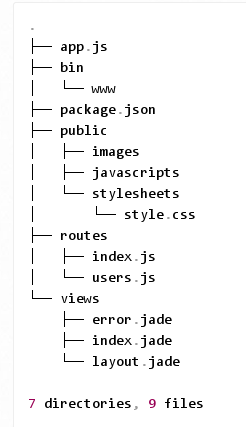
\includegraphics[scale=0.7]{images/estrutura_exp_gen.png}
    \caption{Estrutura criada pelo express-generator \cite{ExpressGen}}
    \label{fig: estrutura criada pelo express-generator}
    \end{figure}

A pasta \textit{public} contém todos os arquivos de imagem, Javascript e CSS que serão enviados para o cliente, como por exemplo os arquivos Javascript do Angular.js, e o arquivo CSS chamado style.css.

Na pasta \textit{views} são definidas as páginas da aplicação, contendo a página do \textit{layout}, do \textit{index}, e uma página de erros. Quando o usuário acessa a aplicação, primeiramente é carregada a página de \textit{layout}, que então carrega a página \textit{index}, e caso algum erro ocorra é enviada uma mensagem de erro.

Para as rotas que definem como serão tratadas as requisições que podem ser realizadas pela aplicação, o \textit{express-generator} cria uma pasta chamada \textit{routes}. Ao receber requisições, o servidor através de funções definidas na pasta \textit{routes}, pode desde renderizar as páginas solicitadas, até encaminhar as requisições para outras rotas, afim de, por exemplo, realizar uma consulta em um banco de dados.

A parte do servidor que o Node.js é responsável, fica no arquivo www da pasta \textit{bin}, e no arquivo app.js na raiz da aplicação.  

Além da estrutura criada pelo \textit{express-generator}, foram criadas mais duas pastas, que são a \textit{models} e a \textit{lib}. Na \textit{models}, ficam os arquivos responsáveis pela conexão e pelos acessos ao MongoDB. A \textit{lib} contém as principais funções da aplicação responsáveis pelo funcionamento do jogo \textit{Math Race}, e da comunicação cliente/servidor, que é feita através do Socket.io, sendo que a sua explicação foi colocada na seção \ref{sec: Socket.io} do apêndice A.

\item[Integração das ferramentas do MEAN \textit{Stack}] \hfill \\
Quando o usuário acessa a aplicação, ocorre uma série de mensagens, entre o lado do cliente e do servidor, afim de informar o servidor que há um novo usuário conectado, e fazer com que o cliente obtenha os dados da partida. 

O diagrama da figura \ref{fig: Diagrama de sequência do acesso da aplicação}, demonstra a sequência de mensagens que ocorrem quando um usuário acessa a aplicação (mensagem 1). 

No lado do servidor, o Node.js envia os arquivos da pasta \textit{public} e o \textit{index} da aplicação (mensagem 2). No lado do cliente, o Angular.js envia uma solicitação de conexão através da função \textit{connect} do Socket.io (mensagem 3), e o Node.js responde com uma mensagem avisando que o usuário está conectado (mensagem 4). Ao receber essa mensagem o Angular.js envia outra mensagem chamada ``\textit{join}'' (mensagem 5), e o Node.js envia os dados referente a operação, a pontuação e o \textit{hall} da fama (mensagem 6, 7 e 8). Por último o Angular.js faz um requisição ao MongoDB para obter o hall da fama atualizado (mensagem 9). 

    \begin{figure}[htb]
    \centering
    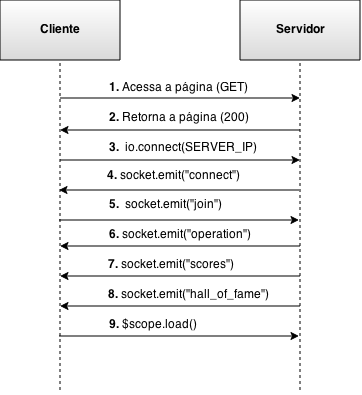
\includegraphics[scale=0.7]{images/diagrama_de_seq_acesso.png}
    \caption{Diagrama de sequência do acesso da aplicação}
    \label{fig: Diagrama de sequência do acesso da aplicação}
    \end{figure}
% codigo do join

A cada final de rodada, o Node.js envia uma nova operação, e o Angular.js envia uma mensagem ao Node.js solicitando o \textit{hall} da fama atualizado. Essa mensagem é enviada através de um módulo do Angular.js chamado \textit{ng-resource}, sendo que através deste módulo é possível interagir com o Node.js utilizando o RESTFul\footnote{ ``RESTful é um serviço web que utiliza o paradigma de arquitetura do REST, ou seja, é o termo normalmente usado para se referir a implementação de Web Services que utilizam tal arquitetura.''\cite{RESTWiki}}. 

Caso o usuário tenha efetuado alguma pontuação na rodada, o Angular.js envia uma mensagem ao Node.js, contendo um objeto JSON com o nome e a pontuação efetuada. O Node.js então faz a inserção no MongoDB, se for um novo usuário, ou atualiza a pontuação, se o nome do usuário já estiver cadastrado no MongoDB, e a nova pontuação for maior do que a antiga.

% diagrama demonstrando a aplicação em execução
\end{description}

% \begin{lstlisting}
% 	$scope.sendResult = function(item) {
% 		if (item.value) {
% 		    ...
% 			socket.emit('send-server-result', item);
% 		};
% 	}
% \end{lstlisting}

\section{Testes de desempenho}
\label{subsec: Testes de desempenho}
Nesta seção serão apresentados os testes que foram realizados através de duas aplicações, o \textit{Math Race} e o ``Encurtador de URL''. 

No \textit{Math Race}, foi efetuado um teste simples através do envio de um conjunto de requisições para consultas ao banco de dados, obtendo-se o tempo de duração para o servidor responder cada conjunto de requisições, além da média de requisições por segundo.

A aplicação ``Encurtador de URL'' foi implementada em diversos ambientes, definidos na tabela \ref{fig: Ambientes dos testes}, afim de avaliar o consumo da memória, a utilização da CPU, e a quantidade de requisições realizadas por tempo. 

\subsection{Testes na Aplicação \textit{Math Race}}
% Nesta subseção o objetivo é demonstrar o comportamento da aplicação através de um conjunto de testes de envio de requisições e consultas ao banco de dados. 
Os testes foram realizados aumentando gradativamente a quantidade de requisições e requisições concorrentes, afim de verificar a latência de resposta do servidor. A cada requisição é realizada uma consulta no banco de dados para obtenção da lista dos dez primeiros usuários e suas pontuações no \textit{hall} da fama.

Na figura \ref{fig: Lista de objetos retornada pelo MongoDB}, podemos observar parte da lista de objetos retornada pela consulta ao banco de dados, que cada cliente realiza ao acessar a aplicação durante os testes.

    \begin{figure}[htb]
    \centering
    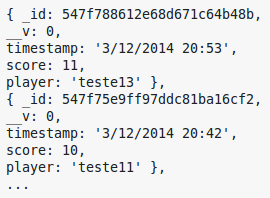
\includegraphics[scale=0.7]{images/objs_hof_bd.png}
    \caption{Lista de objetos retornada pelo MongoDB}
    \label{fig: Lista de objetos retornada pelo MongoDB}
    \end{figure}
% \begin{lstlisting}
% \end{lstlisting}

A máquina utilizada nos testes tem como configurações um Core i7 de 3.6GHZ, e 8GB de memória RAM, utilizando o Fedora 20 de 64 \textit{bits} como sistema operacional.


Na tabela \ref{fig: Carga na quantidade requisições} são mostrados os resultados dos testes realizados na aplicação, através de uma ferramenta específica para teste de carga (\textit{Load test}) conhecida como \textit{weighttp}\footnote{http://redmine.lighttpd.net/projects/weighttp/wiki}. No \textit{weighttp} é possível definir parâmetros como a quantidade de requisições que serão enviadas ao servidor e o número de requisições concorrentes que ocorrerão durante o teste.

Para estes testes foram imaginados dois cenários diferentes, sendo determinada uma quantidade de requisições concorrentes fixa (100 e 1000) em cada cenário. Para cada cenário variou-se a quantidade de requisições de 1.000 até 100.000, obtendo-se o tempo demorado pelo servidor para atender todas estas requisições e a taxa de requisições por segundo. 


\begin{table}[ht]
\centering
\begin{tabular}{|c|c|c|c|}
\hline
\rowcolor[HTML]{CFCFCF} 
\# requisições concorrentes & \# requisições & tempo(seg) & req/seg      \\ \hline
\rowcolor[HTML]{EFEFEF} 
\cellcolor[HTML]{EFEFEF} & 1000 & 0,69 & 1458  \\ \cline{2-4}
\rowcolor[HTML]{EFEFEF} 
\cellcolor[HTML]{EFEFEF} & 2000 & 1,357 & 1472  \\ \cline{2-4}
\rowcolor[HTML]{EFEFEF} 
\cellcolor[HTML]{EFEFEF} & 5000           & 3,437      & 1454  \\ \cline{2-4} 
\rowcolor[HTML]{EFEFEF} 
\cellcolor[HTML]{EFEFEF} & 10000          & 7,690      & 1414  \\ \cline{2-4} 
\rowcolor[HTML]{EFEFEF} 
\cellcolor[HTML]{EFEFEF} & 30000          & 20,928     & 1433  \\ \cline{2-4} 
\rowcolor[HTML]{EFEFEF} 
\cellcolor[HTML]{EFEFEF} & 50000          & 34,986     & 1429  \\ \cline{2-4} 
\rowcolor[HTML]{EFEFEF} 
\cellcolor[HTML]{EFEFEF} & 70000          & 47,102     & 1486  \\ \cline{2-4} 
\rowcolor[HTML]{EFEFEF}
\multirow{-8}{*}{\cellcolor[HTML]{EFEFEF}100} & 100000 & 67,967     & 1471  \\ \hline
    & 1000           & 3,250      & 330   \\ \cline{2-4} 
    & 2000           & 3,350      & 658   \\ \cline{2-4} 
    & 5000           & 3,691      & 1354  \\ \cline{2-4} 
    & 10000          & 7,503      & 1332  \\ \cline{2-4} 
    & 30000          & 21,963     & 1365  \\ \cline{2-4} 
    & 50000          & 37,327     & 1339  \\ \cline{2-4} 
    & 70000          & 52,157     & 1342  \\ \cline{2-4} 
\multirow{-8}{*}{1000}   & 100000         & 74,914     & 1334  \\ \hline    
\end{tabular}
\caption{Carga na quantidade requisições}
\label{fig: Carga na quantidade requisições}
\end{table}

Pode-se notar através da tabela \ref{fig: Carga na quantidade requisições}, que à medida que carga de requisições aumenta, o tempo  total para o servidor responder estas requisições cresce consideravelmente, independentemente do número de requisições concorrentes, mas mantém, em média, a mesma taxa de requisições por segundo. No gráfico da figura \ref{fig: Gráfico de requisições por tempo}, pode-se visualizar de maneira mais clara o comportamento da aplicação, durante a carga de requisições.  
% \newpage
    \begin{figure}[htb]
    \centering
    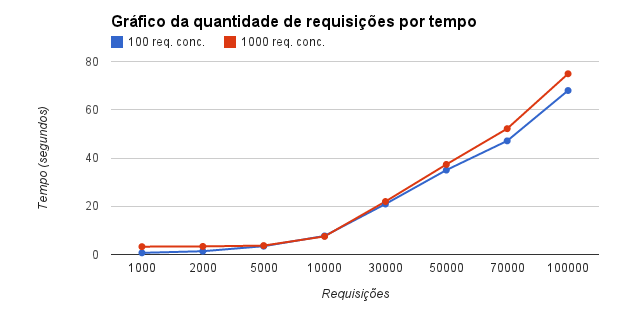
\includegraphics[scale=0.7]{images/reqxtempo.png}
    \caption{Gráfico de requisições por tempo}
    \label{fig: Gráfico de requisições por tempo}
    \end{figure}

\newpage

\subsection{Análise de testes de desempenho do Node.js e do MongoDB com outros ambientes}
Os principais componentes responsáveis pela a escalabilidade no MEAN \textit{Stack} são o MongoDB, através do \textit{autosharding}, e do mapeamento dos dados em memória, e o NodeJS, através do \textit{Event Loop}, e da \textit{Thread Pool}, como mencionado no capítulo \ref{tecnologias}.
    
Existem diversas referências que comparam o desempenho destes dois componentes juntos com outros ambientes, variando desde a linguagem de programação até a base de dados utilizada.

A referência que esta monografia irá utilizar como base é a do artigo de Ricardo Schroeder e Fernando dos Santos,  intitulado ``Arquitetura e testes de serviços web de alto desempenho com Node.js e Mongodb'' \cite{NodejsEMongodb} que implementou um ``Encurtador de URL'' como aplicação.

A aplicação do ``Encurtador de URL'' serve para mapear uma \textit{hash}, de 6 caracteres, para uma URL. Cada \textit{hash} é gerada de maneira única, e aleatória, e foram alocados um milhão de URL's para os testes.

A cada acesso é feita a verificação se a \textit{hash} utilizada é válida.  Primeiro é verificado se a \textit{hash} tem 6 caracteres e depois se ela existe no banco de dados, caso alguma destas verificações falhe é retornado somente um código de  resposta de erro 404. 

Para os testes, a aplicação definida foi implementada em 6 ambientes, que foram descritos na tabela \ref{fig: Ambientes dos testes}. Cada aplicação de um ambiente efetua a mesma requisição e será testada utilizando uma base de amostras contendo duas mil \textit{hashs}. A duração foi estipulada em 60 segundos, sendo que nos  5 segundos iniciais, foram criados quarenta usuários que irão se conectar de maneira incremental, permanecendo ativos durantes os próximos quarenta e cinco segundos e reduzindo durante os dez segundos finais. 

\begin{table}[htb]
\centering
\begin{tabular}{|c|c|c|}
\cline{1-3}
\rowcolor[HTML]{CFCFCF}
Servidor & Linguagem de Programação & Banco de Dados \\ \cline{1-3}
Node.JS  & Javascript               & MongoDB        \\ \cline{1-3}
Node.Js  & Javascript               & PostgresSQL    \\ \cline{1-3}
Netty    & Java                     & MongoDB        \\ \cline{1-3}
Netty    & Java                     & PostgresSQL    \\ \cline{1-3}
Apache   & PHP                      & MongoDB        \\ \cline{1-3}
Apache   & PHP                      & PostgresSQL    \\ \cline{1-3}
\end{tabular}
\caption{Ambientes dos testes \cite{NodejsEMongodb}}
\label{fig: Ambientes dos testes}
\end{table}

Os testes realizados na aplicação foram executados em um ambiente virtualizado contendo as seguintes características: Sistema Operacional CentOS 6.2 x86, 1Gb de memória RAM, 2 núcleos de 2,4Ghz Intel Core I5. A aplicação utilizada para os testes foi o JMeter, que é um software que serve para realizar testes de desempenho, carga e stress, desenvolvido pela Apache\footnote{http://jmeter.apache.org/} . Os resultados são mostrados nas tabelas \ref{fig:graf_memoria}, \ref{fig:graf_cpu} e \ref{fig:graf_tempo}.
\clearpage
\begin{description}
\item[Consumo de Memória RAM] \hfill \\
A memória RAM é um dos princípais pontos de análise em um servidor web, pois está ligada diretamente ao número de requisições que o servidor é capaz de atender em determinado tempo.\cite{NodejsEMongodb}
O resultado do teste demonstrou o uso de memória constante e estabilidade por parte de cada plataforma. Os piores resultados ficaram com os ambientes que utilizam o servidor Apache e a linguagem PHP, enquanto o ambiente que usa Node.js e o MongoDB foi o segundo melhor no índice de consumo de memória.

\begin{figure}[htb!]
\centering
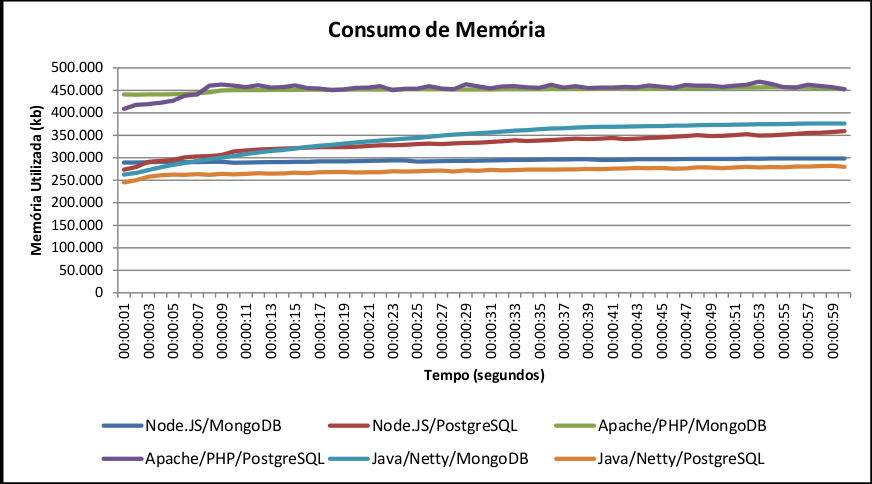
\includegraphics[scale=0.5]{images/graf_memoria.png}
\caption{Consumo de memória RAM durante a execução dos testes \cite{NodejsEMongodb}}
\label{fig:graf_memoria}
\end{figure}

\clearpage
 
\item[Utilização de CPU] \hfill \\
Analisar a utilização de CPU é um fator relevante para que se tenha uma noção da carga gerada pelas requisições efetuadas pelos clientes. Quanto mais próximo de 100\% estiver o uso da CPU, maiores serão as chances do servidor não conseguir atender as requisições recebidas. 

No gráfico da figura \ref{fig:graf_cpu} nota-se um melhor desempenho do Node.js junto ao MongoDB em relação aos outros ambientes, ficando com 40\% de uma média de uso, enquanto em outros ambientes como o que utilizou Java/Netty/PostgreSQL este consumo passou para aproximadamente 90\%.

\begin{figure}[htb]
\centering
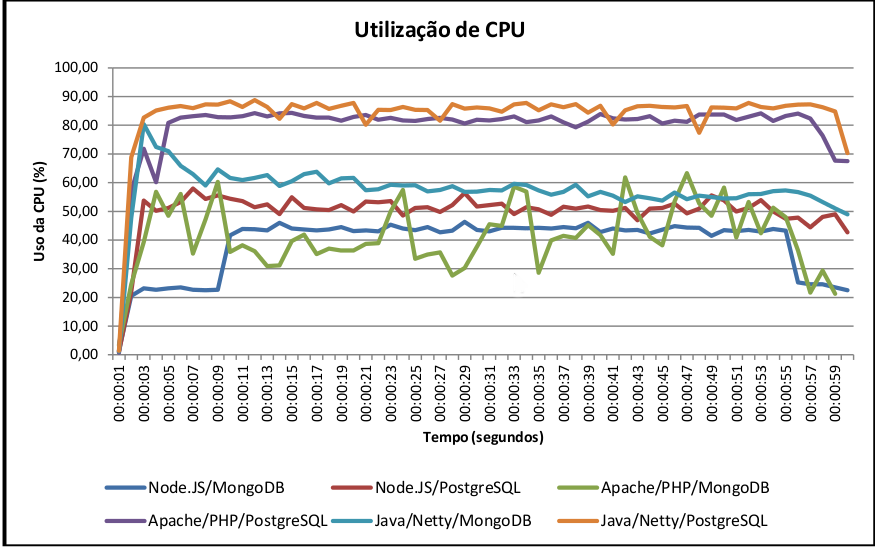
\includegraphics[scale=0.5]{images/graf_cpu.png}
\caption{Consumo de CPU (\%) durante a execução do teste. \cite{NodejsEMongodb}}
\label{fig:graf_cpu}
\end{figure}

% \newpag
\clearpage
\item[Quantidade de requisições por tempo] \hfill \\
O teste de requisições por tempo basicamente indica o quanto de usuários (requisições) o servidor é capaz de absorver.\cite{NodejsEMongodb}

Na figura \ref{fig:graf_tempo} é possível observar que os dois ambientes que mais responderam requisições, que no caso foram o Node.JS/MongoDB e o Netty/MongoDB, utilizaram o mesmo banco de dados. Mas o crédito desse resultado positivo, também se deve aos servidores de alto desempenho, que possuem como característica atender o maior numero de requisições simultâneas. Outro ponto que chama atenção, é como os ambientes com MongoDB se destacaram sobre os ambientes com PostgresSQL.

% \clearpage
\begin{figure}[htb]
% \centering
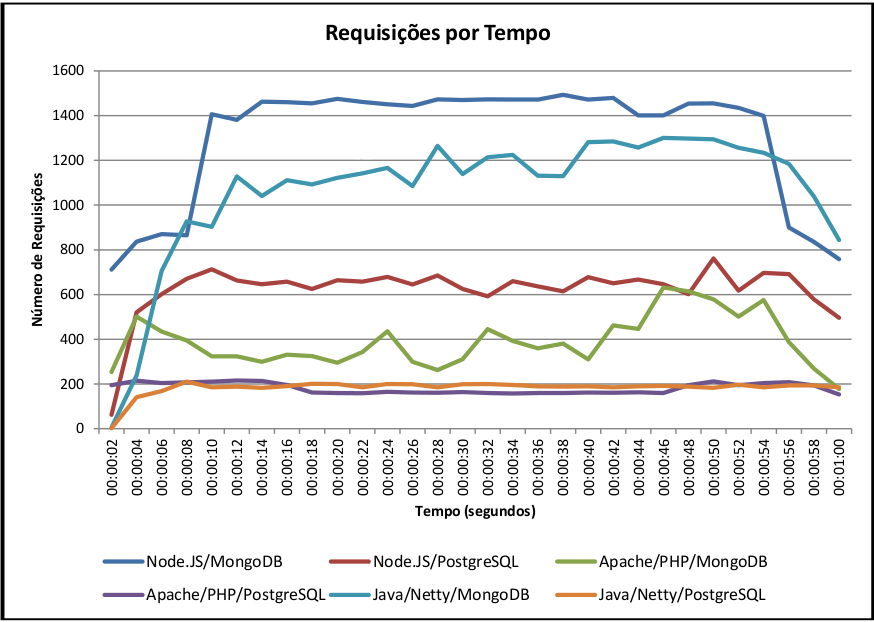
\includegraphics[scale=0.5]{images/graf_req_tempo.png}
\caption{Requisições por tempo. \cite{NodejsEMongodb}}
\label{fig:graf_tempo}
\end{figure}

\end{description}


Após ser realizada uma análise dos testes, tanto no \textit{Math Race} quanto no ``Encurtador de URL'', concluímos que realmente a utilização do Node.js junto ao MongoDB, proporciona um ganho de desempenho considerável, em relação as tecnologias comparadas. Este ganho se deve ao fato das particularidades que cada tecnologia adota, para lidar com escalabilidade, no caso o Node.js com o \textit{Event Loop} e o MongoDb com o \textit{Autosharding}.
%de maneira pura, ou seja, sem que haja alteração para obtenção de resultados  



% PROPOSTA DE DESENVOLVIMENTO

% DIAGRAMA DE CASOS DE USO
%  Especificações dos cs

% DESENVOLVIMENTO DA APLICAÇÃO

% UTILIZAÇÃO DA APLICAÇÃO

%  TESTES DE DESEMPENHO
%   weigthttp
%   objetivo do teste, como foram realizados, hardware utilizado
%      analise dos resultados obtidos

%   figura

% analise dos teste


\chapter{Conclusão}
\label{conclusao}

  Esta monografia apresentou os conceitos e as tecnologias do MEAN \textit{Stack}, além de mostrar como é feita a integração destas ferramentas  para se criar uma aplicação web. Foram apresentados também os resultados de análises com aplicações implementadas neste ambiente, com o intuito de se alcançar uma conclusão sobre a escalabilidade através da utilização das ferramentas do MEAN \textit{Stack}.
  
 Através da análise dos resultados propostos foi concluído que o MEAN \textit{Stack} é de fato uma ótima opção para o desenvolvimento de aplicações web escaláveis, principalmente através de dois de seus componentes o Node.js e o MongoDB. O Angular.js e o Express.js atuam como facilitadores no processo de desenvolvimento, sem estes componentes, dependendo da complexidade da aplicação, o tempo gasto no desenvolvimento da aplicação do lado do cliente pode aumentar drasticamente, e a utilização do Node.js pode ser consideravelmente mais trabalhosa. 
  
%   Além das facilidades no desenvolvimento como por exemplo todos os componentes do MEAN reconhecerem o javascript.
   
\section{Trabalhos Futuros}
 Para os trabalhos futuros, seria interessante uma abordagem de maneira mais ampla, através da comparação do comportamento de diversas aplicações, com diferentes funcionalidades, e em diversos ambientes como Ruby e Python, além dos que foram utilizados nesta monografia. 

%\input{anexo1.tex}     % se houver anexo

\bibliographystyle{brazil}
\bibliography{bibliografia}
% utilize macros (3 primeiras letras do mes em ingles, minusculas) no seu
% .bib para atribuir o nome do mes em portugues nas referencia,
% se o style for brazil, outros estilos tambem aceitam estas macros
% Ex:
%
% @InProceedings{teste,
%   author =       {Luciano}
%   year =         {2013}
%   month =        {}#sep;
% }
%
\addcontentsline{toc}{chapter}{\MakeUppercase{Bibliografia}}

\chapter{Apêndice A}
\label{apendiceA}


\section{Socket.IO}
\label{sec: Socket.io}
O Socket.io é uma API em Javascript que permite que a comunicação entre o servidor e o cliente ocorra sem dificuldades e em tempo real. Ele abstrai e utiliza o protocolo \textit{WebSocket}\footnote{É um protocolo orientado a eventos que permite abrir uma sessão de comunicação interativa entre o navegador do cliente e o sevidor, sendo possível enviar mensagens para um servidor e receber respostas sem ter que consultar o servidor para uma resposta.},  e também possui outras alternativas caso seja um ambiente que não suporte \textit{WebSocket}.
% \section{Math Race}

% Math Race é um jogo em tempo real desenvolvido pelo iloire, que foi feito utilizando Knockout.js, Socket.io e Node.js.

% A idéia do jogo é realizar uma competição em tempo real para ver qual jogador acertar mais contas de matemáticas em determinado tempo.

% Todos os jogadores possuem o mesmo tempo para responder a mesma serie de contas de matemática básica, o diferencial está em que a conta muda para todos os jogadores após a resposta correta da conta anterior ter sido preenchida.

% % Código fonte da aplicação
 

%\singlespacing
%\makecapadissertacao

\end{document}
